\subsection{Job-level validation and extensions}
\label{sec:res-ext}

\subsubsection{Job-level validation of the fluid workload model}
\label{sec:res-job}

All results so far rely on the fluid model, in which backlog can be worked off on any idle GPU with any parallelism. To
test this assumption, every closed-loop run is replayed by a job-level executor and settled again. Jobs are sampled from
the joint gang-size--run-time distribution of the traces; every 15~min the deviation of each class from its nominal load
in the fluid plan becomes a target number of busy GPUs, and jobs are scheduled by slack (jobs whose slack is shorter than
one step must run) and back-filled towards the class and total targets. Jobs are rigid: they run as whole gangs at
nominal speed and cannot be accelerated. A pause costs a checkpoint before it (base: 1~min, during which the GPUs still
draw power) and a restart after it (base: 5~min of powered, unproductive time), with a minimum pause of 15~min; these
values follow asynchronous and in-memory checkpointing~\cite{wan2025,wang2023gemini,hu2024acme}. Deviations of the busy
GPUs from the fluid plan are converted into IT power, the cooling deviation is taken up by the electric chillers, and the
storage and gas engine follow the fluid plan.

On the PAI case day (\figref{fig:jobsim}(a)), the fluid plan of JR-D schedules large catch-up after each event (about
$+3$~MW of IT power after E1 and $+3$ to $+5$~MW after E3), mainly of long jobs. Rigid jobs cannot do this: 11,543
GPU$\cdot$h of the planned catch-up cannot be executed, the slack of the jobs is exhausted before E3, and E3 achieves
only 3.7~MW (below the validity threshold of 4.8~MW), so that E3 becomes invalid and the cost rises from 22.84 to
$30.98\times10^4$~CNY (+36\%). The other five strategies also lose at least one event at job level. With the rigid-job
bound \eqref{eq:rigid}, the plan of JR-D changes: E1 mainly pauses medium jobs, E2 medium and long jobs, and E3 all long
jobs, whose backlog (about 3,900~GPU$\cdot$h) is carried into the next day and worked off after their nominal ends
(\figref{fig:jobsim}(b)). The planned cost rises to $25.15\times10^4$~CNY (+10\%), because catch-up in the gaps is no
longer available, and the job-level cost is $26.52\times10^4$~CNY (+5.4\%, mostly pause and restart overheads) with all
three events valid, a tracking error of the grid import of 0.22~MW and only 397~GPU$\cdot$h of planned catch-up left
unexecuted.

\begin{table}[!t]
\caption{Job-level execution on 52 operating days.}
\label{tab:jobsim}
\centering\footnotesize
\setlength{\tabcolsep}{2.5pt}
\begin{tabular}{@{}lccc@{}}
\toprule
\makecell[l]{Load $\cdot$ recovery\\model of the plan} & \makecell{All events valid:\\JR-D / best IR} & \makecell{Job-level cost of JR-D\\vs best IR} & \makecell{JR-D job-level\\vs fluid cost}\\
\midrule
PAI $\cdot$ fluid & 5.8\% / 0\% & $-4.7\%$ (IR-P, 52/52) & +34.9\%\\
PAI $\cdot$ rigid & 86.5\% / 46--60\% & $-3.0\%$ (IR-P, 50/52) & +6.9\%\\
Acme $\cdot$ fluid & 65\% / 33--35\% & $-7.8\%$ (IR-P, 50/52) & +30.7\%\\
Acme $\cdot$ rigid & 98\% / 75--87\% & $-5.0\%$ (IR-O*, 51/52) & --\\
\bottomrule
\multicolumn{4}{@{}p{0.97\columnwidth}@{}}{\scriptsize Best IR: IR-O* and IR-P; numbers of days on which JR-D is cheaper in brackets; paired $p\le10^{-9}$.}
\end{tabular}
\end{table}

\begin{figure*}[!t]
\centering
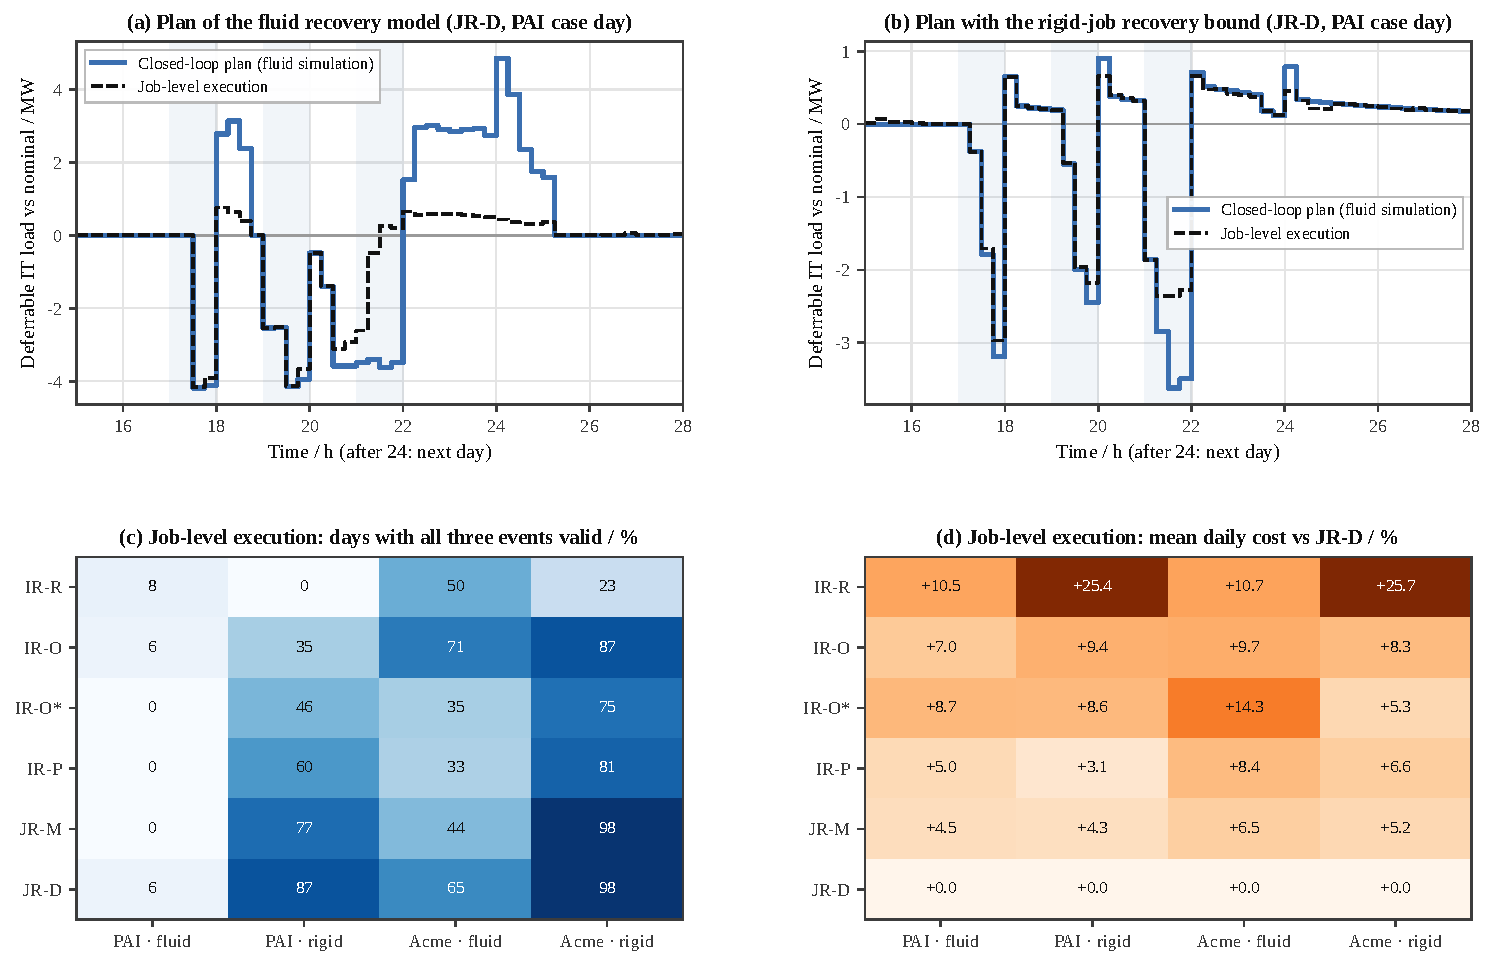
\includegraphics[width=0.90\textwidth]{fig22_jobsim.pdf}
\caption{Job-level validation. (a)(b) Closed-loop plan and job-level execution of JR-D on the PAI case day (deferrable
IT load relative to nominal) with (a) the fluid recovery model and (b) the rigid-job recovery bound; (c)(d) share of the
52 days with all events valid and mean daily cost relative to JR-D at job level.}
\label{fig:jobsim}
\end{figure*}

On the 52 days (\tabref{tab:jobsim}, \figref{fig:jobsim}(c)(d)), the fluid model proves too optimistic for rigid long
jobs: plans made with it fail at job level almost every day with the PAI load (no strategy keeps all events valid on
more than 8\% of the days) and underestimate the cost by 11--38\%; with the Acme load, where long jobs carry 80\% of the
work, all events remain valid on only 33--71\% of the days. The rigid-job bound makes the plans executable: JR-D keeps
all events valid on 98\% of the days with the Acme load and on 86.5\% (instead of 5.8\%) with the PAI load, with a
tracking error of about 0.2--0.3~MW, and the job-level cost of the same strategy is 12--16\% lower when planned with the
rigid model (JR-D: 22.13 against $25.12\times10^4$~CNY per day for Acme, 26.13 against 30.39 for PAI). The advantage of
joint recovery persists at job level: it widens to 4.7--7.8\% with fluid plans and is 5.0\% (Acme) and 3.0\% (PAI) with
rigid plans, not less than the 2.9--3.1\% of the fluid evaluation. The rigid jobs restrict catch-up in the gaps, so more
of the channel can only recharge storage, at efficiency $\eta$; independent recovery relies on catch-up in the gaps to
free the virtual storage and suffers more, whereas joint recovery carries the long-job backlog beyond the last event. In
the rigid variant the fluid accounting by arrival batches reports overdue work that does not exist (46--638
GPU$\cdot$h$\cdot$h for Acme), because the tails of finishing delayed jobs supply catch-up that the first-order bound
$B/\tau_c$ omits; the job-level results, with zero overdue work, are therefore authoritative for this variant. On its
own, the LLM-era Acme load leaves the conclusions of the fluid model unchanged: JR-D is 3.1\% cheaper than IR-P (52/52
days, $p=3.5\times10^{-10}$), similar to the 2.9\% with PAI, with all events valid on 100\% against 98\% of the days.

\begin{figure*}[!t]
\centering
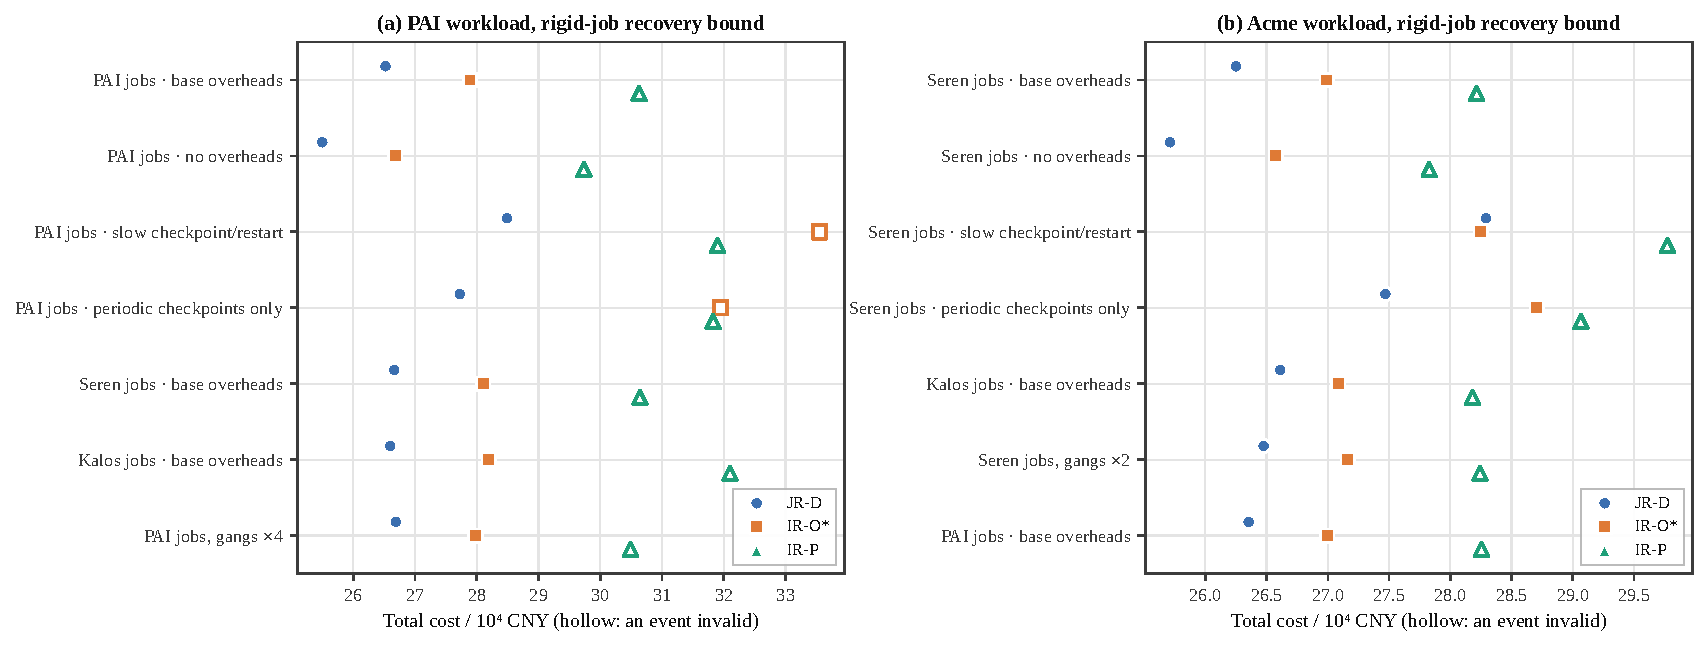
\includegraphics[width=0.90\textwidth]{fig23_jobmix.pdf}
\caption{Job-level total cost on the case day for different job mixes and pause overheads (rigid-job recovery bound;
hollow markers: at least one event invalid).}
\label{fig:jobmix}
\end{figure*}

The job mix and overheads are varied on the case day in \figref{fig:jobmix}: jobs from Seren or Kalos (pre-training
jobs with 512--1,024 GPUs), gang sizes scaled by 2 or 4, and no, base, slow (10-min checkpoint, 15-min restart, 30-min
minimum pause) or periodic-only checkpointing (every 30~min, losing the progress since the last checkpoint). Plans made
with the rigid model are executable in all settings: in all 14 load--job combinations JR-D keeps all three events valid
and is the cheapest in 13; the exception is the Acme load with slow checkpoint and restart, where IR-O* is 0.15\% cheaper
with all events valid as well. With the PAI load the job-level cost exceeds the fluid evaluation by 1.4\% without
overheads, 5.5\% with base overheads and 13\% with slow ones. The strongest benchmarks are more sensitive to overheads:
with the PAI load and slow checkpointing IR-O* keeps only one event valid (two with periodic checkpointing only), and IR-P
loses at least one event in every setting (two with Kalos jobs); with base overheads JR-D is 4.9\% (PAI) and 2.7\%
(Acme) cheaper than IR-O* at job level. With base overheads a day sees 650--4,100 pauses (more with small jobs), about
1,100--1,400~GPU$\cdot$h of restarts and 220--300~GPU$\cdot$h of lost checkpoint progress, together about 1.3--1.6~MWh,
which raises the daily cost of JR-D by 2--4\%; slow checkpointing roughly triples these overheads. Gang granularity
matters little: even when the largest paused job draws 0.7--1.2~MW, the cost of JR-D changes by only 0.3--1.4\%, since
the executor back-fills with small jobs and other classes absorb the granularity error. All pauses at the start of an
event complete within the same minute, so the deferrable IT power steps by about 3--4~MW within 1~min; if the grid
limits ramps, the pauses can be staggered over a few minutes or the IT ramp limit of \secref{sec:computing} can be
imposed. Power swings of synchronous training at the second and iteration scale~\cite{choukse2025} are outside the 15-min
scheduling considered here.

\subsubsection{Pause overheads and multi-level power capping}
\label{sec:ext-overhead}

The fluid model is extended by the pause overhead $o_c$ of \eqref{eq:backlog} (base: 6~min per newly paused GPU for a
1-min asynchronous checkpoint and a 5-min restart; slow: 25~min for synchronous checkpoints and slow restarts of large
models) and by power capping with one level (power $-30\%$, throughput $-12\%$) or three levels ($-15/-30/-45\%$ power
for $-3/-12/-30\%$ throughput), with uniform 6~MW, re-tuned benchmarks and 26 days (\tabref{tab:overhead},
\figref{fig:ext}(a)).

\begin{table*}[!t]
\caption{Pause overheads and multi-level power capping (26 days, uniform 6~MW).}
\label{tab:overhead}
\centering\footnotesize
\setlength{\tabcolsep}{6pt}
\begin{tabular}{@{}lcccc@{}}
\toprule
Setting & \makecell{JR-D cost\\($10^4$~CNY)} & \makecell{JR-D vs\\IR-P} & \makecell{All valid\\JR-D/IR-P/IR-O*} & \makecell{Overhead (GPU$\cdot$h)\\JR-D/IR-P/IR-O*}\\
\midrule
Base (fluid) & 22.50 & $-2.8\%$ (25/26) & 100/96/92\% & --\\
Overhead 6~min & 23.20 & $-2.6\%$ (25/26) & 96/88/62\% & 1,465/1,761/2,919\\
Overhead 25~min & 24.10 & $-2.3\%$ (24/26) & 100/81/27\% & 3,869/4,686/5,624\\
One capping level & 21.87 & $-4.8\%$ (26/26) & 100/62/65\% & --\\
Three capping levels & 21.83 & $-4.5\%$ (26/26) & 100/65/65\% & --\\
Three levels + 6~min & 22.55 & $-2.6\%$ (22/26) & 96/58/38\% & 1,169/1,111/244\\
\bottomrule
\multicolumn{5}{@{}l@{}}{\scriptsize Paired Wilcoxon $p<4\times10^{-4}$ in all settings.}
\end{tabular}
\end{table*}

Pause overheads raise the cost by 3.1\% (6~min) and 7.1\% (25~min), the same order as in the job-level simulation
(2--4\%). JR-D remains the cheapest, with its advantage over IR-P narrowing from 2.8\% to 2.3\%, but the reliability of
the independent benchmarks falls faster: IR-O* keeps all events valid on only 62\% and 27\% of the days. Since the
overhead counts newly paused GPUs, the static split of IR-O*, which pauses and resumes repeatedly between events, incurs
the largest overhead, whereas JR-D defers long jobs continuously and incurs the smallest (half that of IR-O* at 6~min).
Power capping makes every strategy cheaper and widens the advantage of joint recovery: the cost of JR-D falls by 2.8\%
and its advantage over IR-P grows to 4.5--4.8\% (26/26 days). The throughput loss of capping becomes additional
backlog; IR-P keeps all events valid on only 62--65\% of the days instead of 96\%, while JR-D stays at 100\%, consistent
with joint recovery scheduling the backlog left by capping together with the storage deficit across events. Three
levels are only 0.2\% cheaper than one, so a single level of $-30\%$ power for $-12\%$ throughput is nearly sufficient.
With both capping and overheads the two effects largely cancel: JR-D costs $22.55\times10^4$~CNY, close to the base, and
is still 2.6\% cheaper than IR-P (22/26 days); IR-O* then caps more and pauses less (244~GPU$\cdot$h of overhead) but
keeps all events valid on only 38\% of the days.

\subsubsection{Green-power direct supply with offshore wind}
\label{sec:ext-wind}

Offshore wind from the Rudong site is connected behind the meter without grid export under the green-power
direct-connection policy~\cite{ndrc2025green}, which requires the self-consumed share to be at least 60\% of the usable
generation and at least 30\% (35\% before 2030) of the user's consumption. The connection limit stays at 16.0~MW, the
day-ahead wind forecast has an error of 15\% of the capacity (root mean square), and each operating day re-solves the
day-ahead commitment and the IR-P price with its own forecast (\tabref{tab:wind}, \figref{fig:wind}). Without DR, the
renewable share of consumption averages 25.6/40.0/58.4/71.9\% at 5/10/20/40~MW of wind, and the self-consumed share stays
at 100\% up to 10~MW and falls to 89.1\% at 20~MW and 65.5\% at 40~MW. The policy evaluates both shares annually; on
average about 7~MW of wind meets the 30\% share and 40~MW still meets the 60\% self-use, while on a daily basis both
are met on most days at 20~MW (94\%; 91\% with the 35\% threshold), so a wind capacity of about 1.25 times the connection
limit matches the policy best.

\begin{table*}[!t]
\caption{DR with behind-the-meter offshore wind (26 operating days).}
\label{tab:wind}
\centering\footnotesize
\setlength{\tabcolsep}{6pt}
\begin{tabular}{@{}ccccccc@{}}
\toprule
\makecell{Wind\\(MW)} & \makecell{Wind\\(MWh/d)} & \makecell{Commitment sum\\(MW, declared)} & \makecell{JR-D DR revenue\\($10^4$~CNY/d)} & \makecell{JR-D cost\\($10^4$~CNY)} & \makecell{JR-D vs\\IR-P} & \makecell{All valid\\JR-D/IR-P/IR-O*}\\
\midrule
0 & 0 & 17.7 (100\%) & 6.21 & 22.46 & $-2.5\%$ & 100/96/96\%\\
5 & 50 & 13.4 (96\%) & 4.41 & 18.99 & $-6.6\%$ & 92/58/92\%\\
10 & 100 & 7.8 (92\%) & 2.36 & 16.21 & $-6.6\%$ & 77/46/58\%\\
20 & 199 & 6.6 (100\%) & 2.08 & 10.77 & $-5.9\%$ & 85/73/65\%\\
\bottomrule
\multicolumn{7}{@{}l@{}}{\scriptsize Paired differences: 25/26, 24/26, 24/26 and 21/26 days cheaper; $p$ = $9\times10^{-8}$, $1\times10^{-6}$, $3\times10^{-6}$ and 0.002.}
\end{tabular}
\end{table*}

\begin{figure*}[!t]
\centering
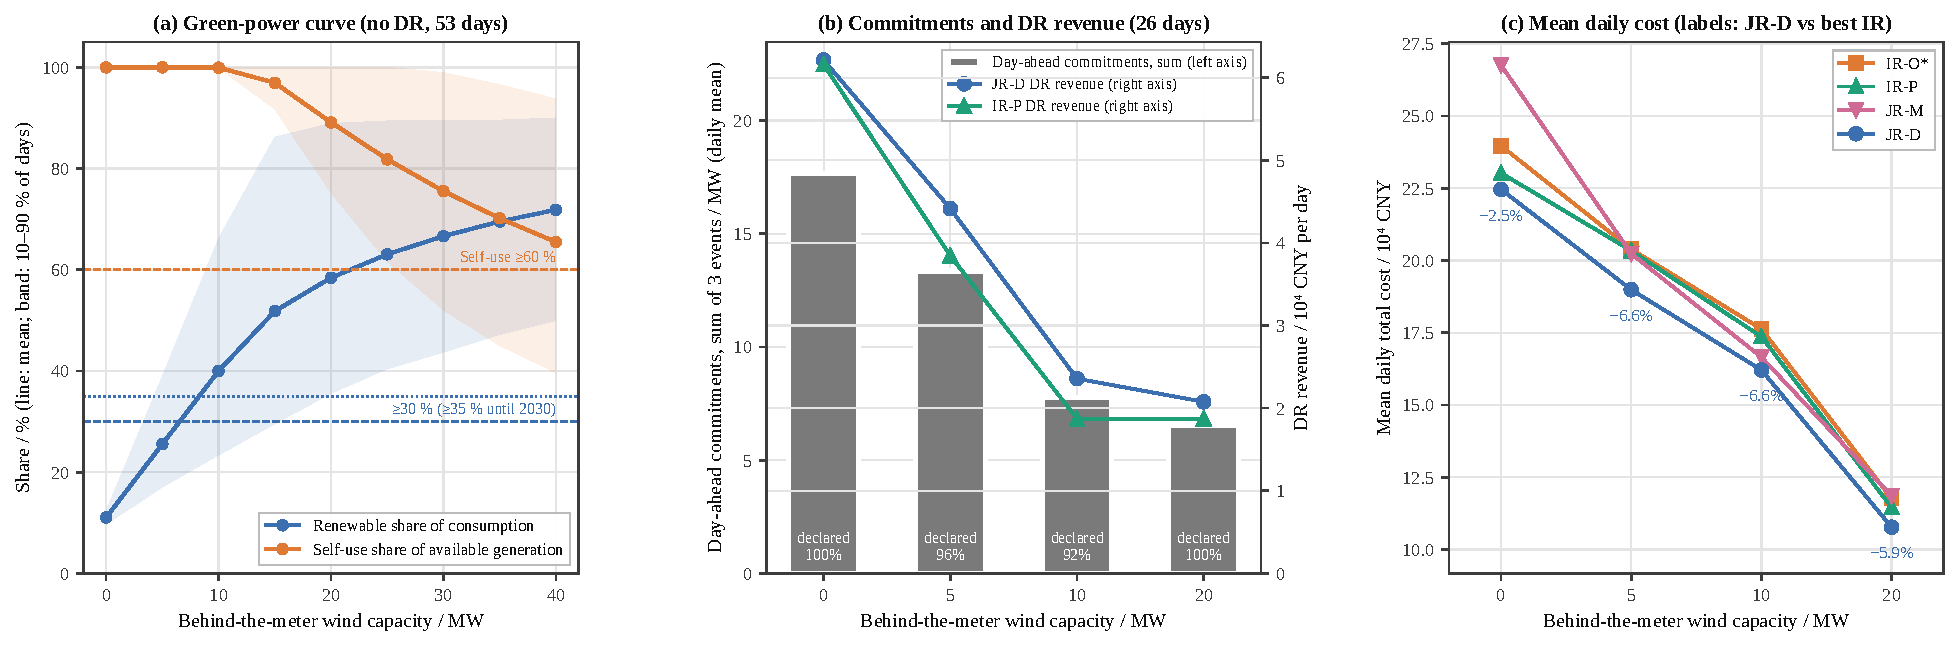
\includegraphics[width=0.98\textwidth]{fig26_wind.pdf}
\caption{Green-power direct supply with offshore wind. (a) Renewable share of consumption and self-used share of the
available generation without DR (lines: means; bands: 10--90\% of the days) with the policy thresholds; (b) sum of the
day-ahead commitments (bars; share of declared events inside) and DR revenue; (c) mean daily cost (labels: JR-D
relative to the strongest independent benchmark).}
\label{fig:wind}
\end{figure*}

The meter-based baseline makes the deliverable commitments fall quickly with the wind capacity. The baseline is taken
from the meter data of the reference days and thus inherits their wind; once the wind of the operating day deviates from
that average, the metered ``reduction'' deviates as well even if the load does not. The total commitment falls from 17.7
to 6.6~MW at 20~MW of wind ($-63\%$), the DR revenue of JR-D drops to one third, and on days with little forecast wind the
day-ahead model declares some events with zero commitment (8\% of the events at 10~MW). The saved electricity cost far
exceeds the lost DR revenue: the daily cost of JR-D falls from 22.5 to $10.8\times10^4$~CNY at 20~MW. The advantage of
joint recovery widens with wind, to 5.9--6.6\% against IR-P (2.5\% without wind), because forecast errors shift the net
load during the events and reduce validity for all strategies, but less for joint recovery, which keeps more margin for
corrections by planning backlog and storage across events (all events valid on 77--92\% of the days against 46--73\%
for IR-P). The differences come from days with weak and mispredicted wind, whereas on the windy case day (122 and
244~MWh at 10 and 20~MW) commitments are small and easy to meet and the strategies differ by less than 1\%. Measuring
the baseline at the grid meter thus counts the fluctuations of behind-the-meter wind as response or counter-response
(see~\cite{chao2011} for baseline choice in general); metering the wind separately and settling on the load net of wind
would preserve the flexibility of the data center, which needs clarification at the policy level.

\subsubsection{Winter waste-heat recovery}
\label{sec:ext-heat}

In winter, a water-source heat pump (3~MW$_{\mathrm{el}}$, COP 3.5) lifts the waste heat of the chilled-water return to
a nearby heat network through a hot-water tank \eqref{eq:heat}, with the gas boiler as backup. The case day is the cold
day of 10 January 2025 (daily mean 0.4~$^\circ$C), the heat demand is about 5.3~MW$_{\mathrm{th}}$ (127~MWh$_{\mathrm{th}}$
per day), the connection limit stays at the 15.5~MW without heating, and the 26 coldest winter days are the operating
days (\tabref{tab:heat}, \figref{fig:heat}).

\begin{table*}[!t]
\caption{Winter waste-heat recovery (26 coldest days, uniform 6~MW).}
\label{tab:heat}
\centering\footnotesize
\setlength{\tabcolsep}{6pt}
\begin{tabular}{@{}lccccc@{}}
\toprule
Setting & \makecell{JR-D cost\\($10^4$~CNY)} & \makecell{JR-D vs\\IR-P} & \makecell{All valid\\JR-D/IR-P/IR-O*} & \makecell{Waste-heat share\\JR-D / IR-P} & \makecell{Boiler (MWh)\\JR-D / IR-P}\\
\midrule
Gas boiler only & 28.25 & $-2.1\%$ (25/26) & 100/96/96\% & 0 / 0 & 138.6 / 138.6\\
Heat pump, no tank & 23.56 & $-4.4\%$ (26/26) & 100/69/96\% & 82.6 / 77.4\% & 24.1 / 31.3\\
Heat pump + 20~MWh & 23.56 & $-2.3\%$ (25/26) & 100/96/96\% & 97.1 / 91.4\% & 4.1 / 12.1\\
Heat pump + 40~MWh & 23.88 & $-1.4\%$ (25/26) & 100/96/92\% & 99.9 / 99.4\% & 0.2 / 0.8\\
\bottomrule
\multicolumn{6}{@{}l@{}}{\scriptsize Boiler heat includes the first 6~h of the next day; paired Wilcoxon $p<10^{-5}$.}
\end{tabular}
\end{table*}

\begin{figure*}[!t]
\centering
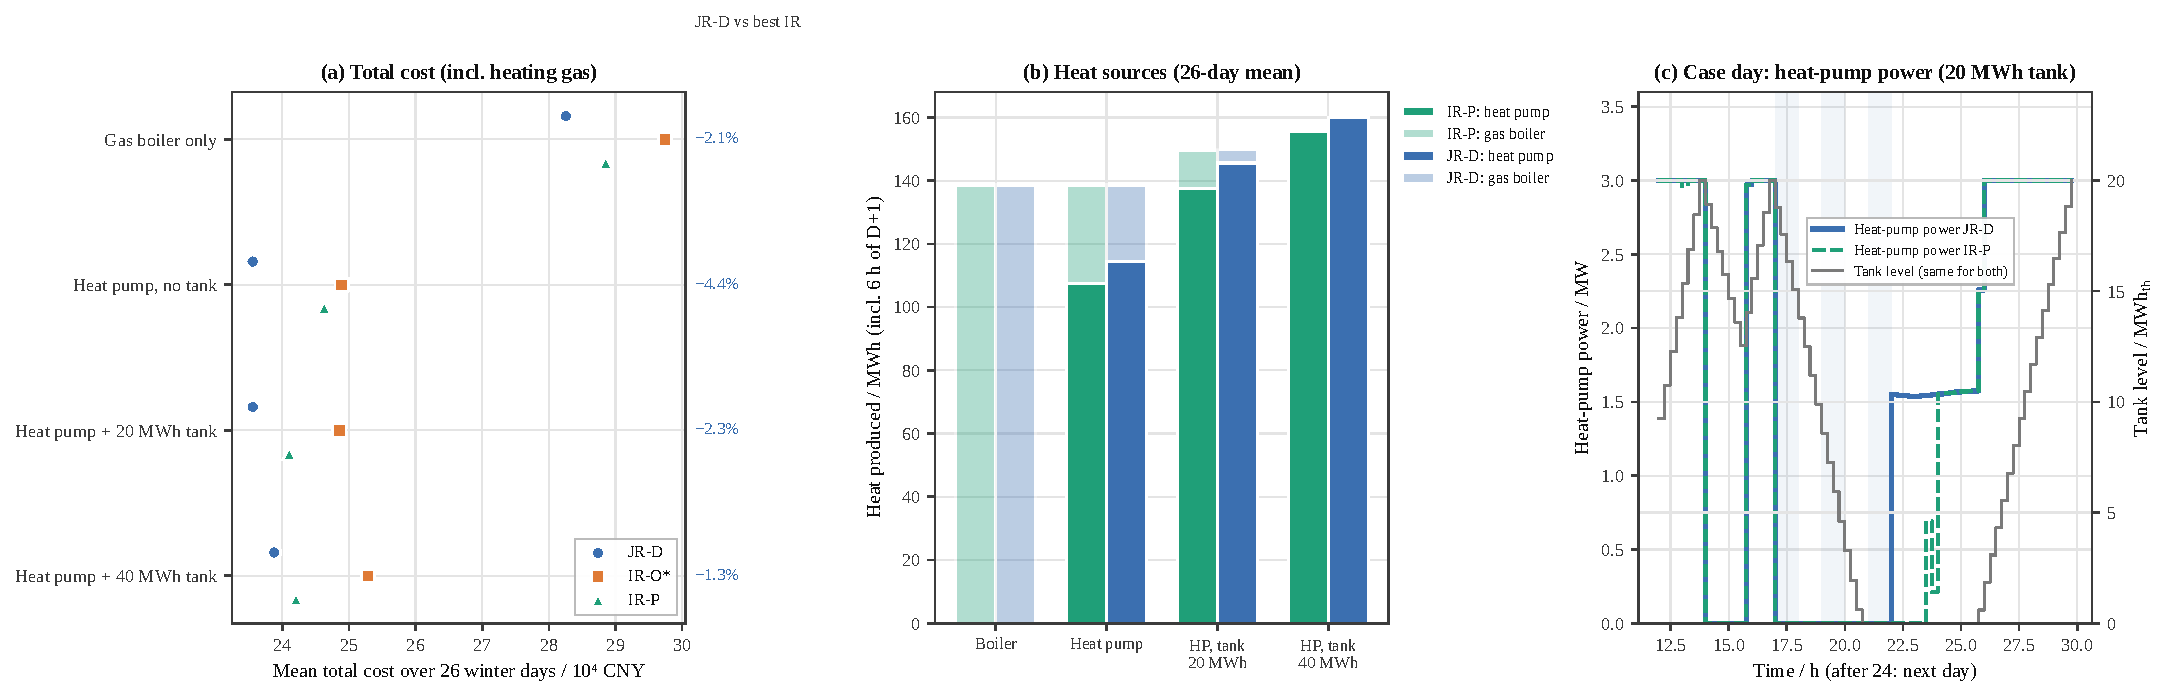
\includegraphics[width=0.98\textwidth]{fig27_heat.pdf}
\caption{Winter waste-heat recovery. (a) Mean total cost on the 26 coldest days including heating gas (right: JR-D
relative to the strongest independent benchmark); (b) heat produced by the heat pump and the gas boiler; (c) heat-pump
power and tank level on the case day with the 20-MWh tank.}
\label{fig:heat}
\end{figure*}

Waste-heat recovery pays off by itself: it lowers the daily cost by 15.5--16.6\% against boiler heating (4.4--4.7$\times
10^4$~CNY per day for JR-D) and the emissions by 16--19~t of CO$_2$ per day. Without a tank, the heat pump competes with
catch-up computing for the channel: its load is part of the baseline, so switching it off during an event counts as
reduction, but the heat demand continues and the heat pump must catch up afterwards, exactly when catch-up computing and
battery recharging need the headroom. The IT side of independent recovery takes this headroom first, so IR-P keeps all
events valid on only 69\% instead of 96\% of the days and burns more boiler gas, while joint recovery, which schedules
the heat pump together with the other states, widens its advantage to 4.4\% (26/26 days). A tank decouples heating from
the events: the heat pump stops during the events, the tank supplies the heat and is recharged afterwards. All strategies
then keep the events valid on 96--100\% of the days and the advantage returns to 2.3\%, but joint recovery recovers about
6 points more waste heat (boiler heat 4.1 against 12.1~MWh), because after E3 it gives the headroom to the heat pump
first whereas independent recovery gives it to catch-up computing (\figref{fig:heat}(c): JR-D restarts the heat pump right
after E3, IR-P about 1.5~h later, with the boiler covering the gap). A larger tank is not always better: the 40-MWh tank
already shifts all peak-period heat-pump load to the valley hours in normal operation, which lowers the baseline in the
event hours by about 0.7~MW against no tank and 0.3~MW against the 20-MWh tank (the same mechanism as for large
batteries in \secref{sec:res-capacity}); JR-D then costs 1.4\% more than with the 20-MWh tank and its advantage shrinks to
1.4\%.

\subsection{Discussion}
\label{sec:discussion}

The results support three practical implications. First, consecutive DR should be bid and settled as a whole: the
capability region of joint recovery is described by the stand-alone capabilities and one cross-event energy budget, and
declaring these virtual-battery parameters instead of one value per event lets the grid operator call more capacity with
the same reliability. Second, the main value of joint recovery lies in the reliably deliverable capacity rather than in
the operating cost at moderate commitments, and it is largest when the recovery channel is scarce: hot evening peaks,
short gaps, tight connection margins, liquid cooling, smaller batteries or a heat pump without a tank. Third, joint
recovery can be implemented without merging the IT and facility control systems, through a few plan--price exchanges per
15~min, whereas a one-shot price signal is insufficient. The settlement rules matter as well: the rebound charge, the
baseline method with storage arbitrage and behind-the-meter wind, and ramp requirements change what the data center
can deliver and should be designed together with its flexibility.

The study has limitations. The fluid workload model is optimistic for rigid gang-scheduled jobs; the rigid-job bound is
a first-order approximation, and the job-level executor is a slack-based heuristic without job dependencies, network
topology or communication overheads. The PAI trace predates LLMs and the Acme trace stems from one institution, while
frontier pre-training jobs may use thousands of GPUs. Only the call of the last event is uncertain, the scenario sets are
small and deterministic, and the ambiguity set covers only the scenario probabilities (a Wasserstein
ball~\cite{esfahani2018} would also cover unseen outcomes). The capability region is computed under perfect information.
The distributed scheme approximates the proximal term by tangent cuts and does not model communication delays, losses,
asynchronous updates or strategic behaviour. Thermal inertia, policy and waste-heat parameters take typical values, the
wind forecast errors are synthetic, the season and climate tests replace only the weather, and the system is aggregated
on one bus without distribution network constraints.
